\documentclass[8pt]{article}
\usepackage{graphicx}
\usepackage{float}
\usepackage{listings}
\lstset{language=bash, xleftmargin=0.5cm}

\setlength{\topmargin}{0.0in}
\setlength{\headheight}{0in}
\setlength{\headsep}{0in}
\setlength{\textheight}{9in}
\setlength{\textwidth}{6.5in}
\setlength{\oddsidemargin}{.0in}
\setlength{\evensidemargin}{.0in}
\setlength\parindent{0pt}

\begin{document}

\section{Lego Reactor Demo}

The Lego Reactor Demo package consists of a point kinetic reactor model with GUI frontend which interfaces with an Arduino driven Lego model (optional).  This package was developed to inform young students about nuclear engineering. Control rod movement and reactor power visual feedbacks are presented to the audience via servo and LED control respectively.

\subsection{Software}

In order to run the pyReactor GUI program, the user must first install the following prerequisites:

\begin{itemize} \itemsep0em
\item python2.7
\item numpy
\item scipy
\item matplotlib
\item wxpython
\item pyserial
\end{itemize}

On an Ubuntu Linux machine, for example, the following commands should install all of the prerequisites for you:

\begin{lstlisting}
sudo apt-get update && apt-get install build-essential python2.7 \
python-pip libblas-dev git python-setuptools
sudo pip install pip --upgrade
sudo pip install numpy scipy matplotlib wxpython pyserial
\end{lstlisting}

Once all prerequisites have been installed, you may grab the python source code and install the reactor GUI program on Linux or OSX:

\begin{lstlisting}
git clone https://github.com/wgurecky/pyReactor.git
cd  pyReactor
python setup.py develop
\end{lstlisting}

The GUI executable can now be evoked from the command line:
\begin{lstlisting}
pyReactor
\end{lstlisting}

\begin{figure}
\centering
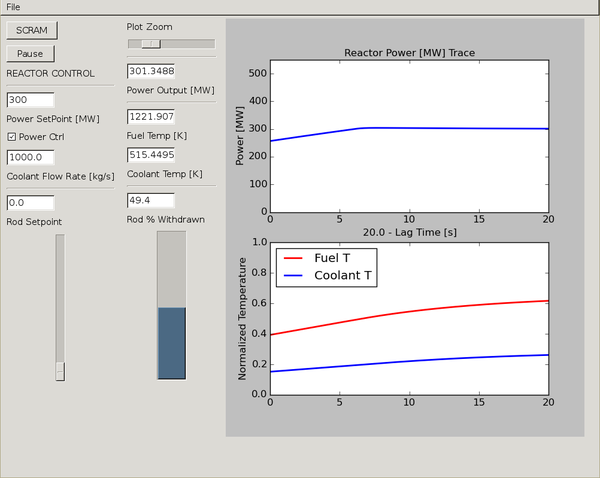
\includegraphics[scale=0.4]{../simulator_screenshot.png}
\caption{The reactor GUI application.}
\end{figure}

\subsection{GUI Operation}

The reactor can be operated in two modes which may be toggled by clicking the $Pwr\ Ctrl$ checkbox in the GUI. In power control mode reactor will attempt to maintain the user set power.  To set a power level, first make sure the $Pwr\ Ctrl$ toggle is checked, then type in a value from 0-500 in the $Power\ Set\ Point$ field and press enter.  \\

In standard control rod based mode ($Pwr\ Ctrl$ toggle unchecked), the rod position may be set with a vertical slider. The rods move at a set, relatively slow pace. The rod height is visualized by a vertical bar plot. \\

The coolant flow rate can be adjusted by typing in an integer value into the $coolant\ flow\ rate$ field followed by pressing enter. \\

Temperature is plotted as a dimensionless distance to the SCRAM value. This is done to display both the fuel and moderator temperature on the same plot. \\

The scram button will generate a SCRAM event. To unlock the reactor after a SCRAM, click the SCRAM button again. \\

An Arduino may be connected to the computed via USB. The Arduino play included in this software package will automatically attempt to establish a connection to the Arduino. The Arduino code controls a small servo which is used to raise/lower control rods. It also drives a blue LED to give visual reactor power feedback.

\subsection{Hardware}

To connect the Arduino with the Lego reactor, ensure to follow the following diagram: \\

\begin{figure}[h]
\centering
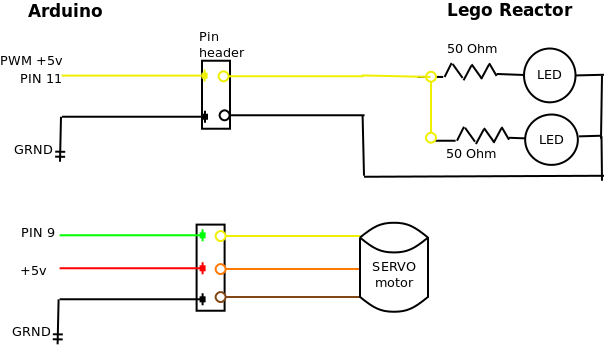
\includegraphics[scale=0.5]{wire_dia.png}
\caption{Reactor wiring diagram.}
\end{figure}

$WARNING$:  When connecting the wires to the Lego model only do so by handling the wires from the black shrink wrap tips.  The wires easily pull out of their shrink wrap pin tips.  

\subsection{Construction Notes}

Tips in case anything needs to be repaired.

\subsubsection{Control rod drive}

4 control rods are coupled to a center drive shaft in a Rod Cluster Control Assembly (RCCA).  The center drive shaft is friction fitted to the control rod assembly.  This fitting is easily decoupled. The control rods are guided by clear straw tubes as they travel up and down. \\

The servo is geared to a (in)1:9(out) ratio.  The servo only has 180 degrees of operating range.  One end of a fishing line is glued to a pulley on the output shaft and the other is attached to the RCCA drive shaft. \\

$WARNING$:  When removing the control rod drive gearbox from the top of the reactor  disconnect the RCCA drive shaft from the control rod assembly first!  Otherwise you risk breaking the fishing line.

\subsubsection{LEDs}

The LEDs are wired in parallel with 50 ohm current limiting resistors.  They are positioned inside the bottom of the control rod guide tubes facing upwards.

\subsubsection{Fuel Elements}

The fuel and control rods are spray painted bamboo skewers to keep costs low.  To prevent them from falling through the spacer grids, they are cut to length and are capped with a small piece from a plastic straw and a small amount of hot glue.

\subsubsection{Reactor Vessel}

The top end cap can be carefully removed to add or remove fuel elements from the core.  To improve the structural integrity of the vessel the brick in the barrel could be ``welded" together using Acetone in the future.

\end{document}